\begin{frame}[c]{Motivation}
  \begin{center}
    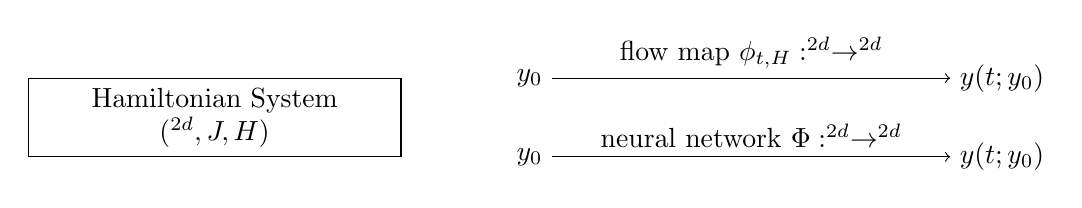
\begin{tikzpicture}
      \node [draw,text width=4.5cm,align=center] at (0,-0.5)
          {Hamiltonian System\\ $(\R^{2d}, J, H)$};

      \node (y0) at (4,0) {$y_0$};
      \node (yt) at (10,0) {$y(t; y_0)$};

      \draw [->] (y0) edge node[above]{flow map $\phi_{t,H} : \R^{2d} \to \R^{2d}$} (yt);

      \node (y01) at (4,-1) {$y_0$};
      \node (yt1) at (10,-1) {$y(t; y_0)$};

      \draw [->] (y01) edge node[above]{neural network $\Phi : \R^{2d} \to \R^{2d}$} (yt1) ;
    \end{tikzpicture}

    \vspace{0.3cm}
    \bemph{Idea:} Use symplectic neural networks.
  \end{center}

  \vspace{0.3cm}
  One possible architecture recently proposed by \citeauthor{Jin2020}\footcite{Jin2020}
  \bemph{Own work:}
  \begin{itemize}
    \item Implementation in PyTorch.
    \item Extension to high-dimensional Hamiltonian systems 
    (discretized PDEs) via convolution.
    \item Improve performance with batch normalization.
  \end{itemize}
\end{frame}

\begin{frame}{Structure}
  \tableofcontents
\end{frame}

\section{Neural network ~\newline basics}

\begin{frame}{Neural network}
  \begin{definition}[Neural network]
    A neural network $\Phi$ is a composition of one or multiple layers $\phi$ 
    with compatible input and ouput dimensions:
    \begin{equation*}
      \Phi(x;\Theta) = \phi_{n_L} \lb \phi_{n_L-1} \lb \cdots
      \lb \phi_2(
      \phi_1(x;\theta_1); \theta_2 ) \cdots \rb ; \theta_{n_L-1} \rb ; \theta_{n_L} \rb
    \end{equation*}
    We denote the vector of
    \bemph{all layer parameters} with $\Theta = (\theta_1^\top, \dots, \theta_{n_L}^\top)^\top$.
  \end{definition}
  
  Example: so-called (fully-connected) linear layer
  \begin{equation*}
    \phi(x) = Wx +b
  \end{equation*}
  with parameters $W \in \R^{n_2 \times n_1}$ 
  and $b \in \R^{n_2}$,\\
  i.e. $\theta = (vec(W)^\top, b^\top)^\top \in \R^{n_2 n_1 + n_2}$.
\end{frame}

\begin{frame}{Training data and loss}
  Here: supervised learning

  \begin{block}{Training data}
    $\mathcal{T} = \{(x_1, y_1) \dots, (x_{n_{\text{train}}},y_{n_{\text{train}}}) \}
   \subset \R^{n_x} \times \R^{n_y}$
  \end{block}

  \begin{block}{Loss}
    \begin{equation*}
      L(\mathcal{T}, \Theta) = 
      \sum_{(x_i, y_i) \in \mathcal{T}} \norm{\Phi(x_i; \Theta) - y_i}^2_2
    \end{equation*}
  \end{block} 

  \vspace{0.3cm}
  \bemph{Goal:} Solve optimization problem $\min_\Theta L(\mathcal{T}; \Theta)$
\end{frame}

\begin{frame}[c]{Gradient descent}
  \bemph{Goal:} Solve optimization problem $\min_\Theta L(\mathcal{T}; \Theta)$
  \vspace{0.3cm}

  learning rate $\gamma \in  \R$

  epoch $i \in \N$
  \begin{block}{Gradient descent}
    \begin{equation*}
      \Theta_{i+1} = \Theta_i - \gamma \grad[\Theta]{L(\mathcal{T};\Theta_{i})}
    \end{equation*}
  \end{block}

  different gradient descent flavors, for example Adam, ...
\end{frame}

\section{Hamiltonian Systems}

\begin{frame}{Hamiltonian system}
  \begin{equation*}
    \text{Phase space } \R^{2d},\,
    \text{Poisson matrix } J = \begin{pmatrix}
      0 & I_d \\
      -I_d & 0
    \end{pmatrix}
  \end{equation*}
  \begin{equation*}
    \text{\bemph{Hamiltonian} or \bemph{total energy} }
    H: \mathbb{R}^{2d} \to \mathbb{R}
  \end{equation*}

  \begin{definition}[Hamiltonian (ODE) system]
    Given $(\R^{2d}, J, H)$ and initial values
    $y_0 = (q_0, p_0) \in \mathbb{R}^{2d}$ for time $t_0 \in I$, 
    find a solution 
    \begin{equation*}
      y: I \subset \mathbb{R} \to \mathbb{R}^{2d},\, t \mapsto y(t) =
      \left(
      \begin{array}{c}
        q(t)\\
        p(t)
      \end{array}
      \right)\hspace{-5pt}
      \begin{array}{l}
        \text{coordinates}\\
        \text{momenta}\\
      \end{array}
    \end{equation*}
    such that
    \begin{align*}
      \dot{y}(t) &= J \grad{H}(y(t)) \quad \text{for } t \in I \subset \mathbb{R} \\
      y(t_0) &= y_0
      .
    \end{align*}
  \end{definition}
  \nocite{hairer2006}
\end{frame}

\begin{frame}[c]{Conservation of the total energy}
  \centering
  \begin{equation*}
    \ddt H(y(t)) = \lsb \grad{H}(y(t)) \rsb^\top \dot{y}(t) = 
    \lsb \grad{H}(y(t)) \rsb^\top J \grad{H}(y(t)) = 0
  \end{equation*}
\end{frame}

\begin{frame}{Flow}
  flow of a Hamiltonian system
  \begin{equation*}
    \phi_{t,H}\begin{pmatrix}
      q_0 \\
      p_0
    \end{pmatrix}
    = \begin{pmatrix}
      q(t; q_0, p_0) \\
      p(t; q_0, p_0)
    \end{pmatrix}
  \end{equation*}

  \begin{definition}
    A differentiable map $\phi : U \to \mathbb{R}^{2d}$ (where $U \subset \mathbb{R}^{2d}$ is an open set)
    is called symplectic if for the Jacobian matrix $\jac{\phi}{x}$ holds everywhere that
    \begin{equation*}
      \lb \jac{\phi}{x} \rb^\top J \lb \jac{\phi}{x} \rb = J
      .
    \end{equation*}
  \end{definition}

  \bemph{The flow $\phi_{t,H}$ of a Hamiltonian system is symplectic!} (Poincaré 1899)
\end{frame}

\section{SympNets: ~\newline Symplectic networks}

\begin{frame}{The building block}
  \begin{definition}[Unit Triangular Layer]
    A layer $\phi : \mathbb{R}^{2d} \to \mathbb{R}^{2d}$ 
    is called a unit triangular layer with \bemph{layer transform}
    \begin{equation*}
      \layertf : \mathbb{R}^d \to \mathbb{R}^d,\, p \mapsto \layertf(p)
    \end{equation*}
    and bias parameter $b \in \R^{2d}$, if the layer $\phi$ can be expressed as
    \begin{equation*}
      \phi_\up \qpvec
      = \begin{pmatrix}
        q + \layertf(p) \\
        p
      \end{pmatrix} + b \quad \text{(upper unit triangular layer)}
    \end{equation*}
    or
    \begin{equation*}
      \phi_\low \qpvec
      = \begin{pmatrix}
        q \\
        \layertf(q) + p
      \end{pmatrix} + b. \quad \text{(lower unit triangular layer)}
    \end{equation*}
  \end{definition}

  \bemph{A unit triangular layer is symplectic iff. the Jacobian of the 
  layer transfrom $\layertf$ is symmetric everywhere.}
\end{frame}

\begin{frame}[c]{Linear layers}
  The (symplectic) \bemph{linear layers} are defined by the layer transform
  \begin{equation*}
    \layertf(p) = Sp
  \end{equation*}
  with a symmetric matrix $S \in \R^{d \times d}$ parametrized\\
  by $A \in \R^{d \times d}$ via $S=A^\top+A$.
  \vspace{1cm}
\end{frame}

\begin{frame}[c]{Activation layers}
  The (symplectic) \bemph{activation layers} are defined by the layer transform
  \begin{equation*}
    \layertf(p) = \lb a_i \activation(p_i) \rb_{i=1}^d
  \end{equation*}

  with:
  \begin{itemize}
    \item an activation function $\activation : \R \to \R$
    \item coefficients $a \in \R^d$ 
  \end{itemize}
\end{frame}

\begin{frame}[c]{Gradient layers}
  The (symplectic) \bemph{gradient layers} are defined by the layer transform
  \begin{equation*}
    \layertf(p) = K^\top \bigg( a_j \activation \lb (Kp)_j + c_j \rb \bigg)_{j=1}^n
  \end{equation*}

  with:
  \begin{itemize}
    \item an activation function $\activation : \R \to \R$
    \item width $n \in \N$ ($n \gg d$)
    \item parameters $a,c \in \R^n$ and $K \in \R^{n \times d}$
  \end{itemize}

  \vspace{0.3cm}
  The layer transform $\layertf$ can approximate a gradient of an arbitrary
  differentiable real-valued function.\footcite{Jin2020}
\end{frame}

\section{Normalization and ~\newline Convolution for ~\newline SympNets}

\begin{frame}[c]{Batch Normalization}
  Initially proposed by \textcite{batchnorm-ioffe15}.

  \bemph{Goal:} Normalize layer input to zero-mean and unit variance.

  \begin{itemize}
    \item Prevent vanishing gradient.
    \item Smooth optimization landscape.\footcite{Santurkar2018}
  \end{itemize}

  Apply batch normalization transform $\eta_{\gamma, \beta}$ 
  right before activation function,\\
  i.e. replace $\activation$ by $\activation \circ \eta_{\gamma, \beta}$
  in the layer transform of the activation layers and gradient layers.
\end{frame}

\begin{frame}[c]{Convolution vs. cross-correlation}
  Given two discrete functions $f,g \in \mathbb{R}^\mathbb{Z}$, discrete
  \bemph{convolution} is defined as 
  \begin{equation*}
    *: \mathbb{R}^{\mathbb{Z}} \times \mathbb{R}^{\mathbb{Z}} \to \mathbb{R}^{\mathbb{Z}},
    \quad (f*g)(\tau) = \sum^{\infty}_{a=-\infty} f(a) g(\tau - a)
    .
  \end{equation*}

  Discrete \bemph{cross-correlation} is defined as
  \begin{equation*}
    \star: \mathbb{R}^{\mathbb{Z}} \times \mathbb{R}^{\mathbb{Z}} \to \mathbb{R}^{\mathbb{Z}},
    \quad (f \star g)(\tau) = \sum^{\infty}_{a=-\infty} f(a) g(\tau + a)
    .
  \end{equation*}
\end{frame}

\begin{frame}[c]{Valid cross-correlation}
  For two discrete functions with finite support (i.e. vectors $\R^n$ for a $n \in \N$), 
  only evaluate the cross-correlation where the support of both 
  discrete functions fully overlaps.
  \begin{equation*}
    \star_{\text{v}} : \mathbb{R}^{n_k} \times \mathbb{R}^{n_x} \to \mathbb{R}^{n_x-n_k+1}
  \end{equation*}

  \vspace{0.3cm}
  \bemph{Example:}
  $k \in \R^3$,
  $x \in \R^6$,
  $y := \star_{\text{v}}(k,x) \in \R^4$

  \vspace{0.3cm}
  \centering
  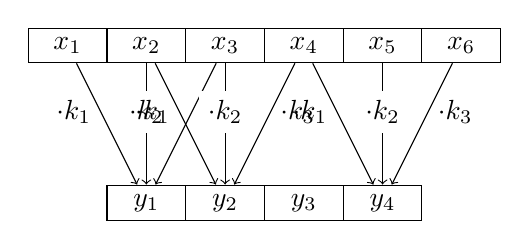
\begin{tikzpicture}
    \foreach \i in {1,2,3,4,5,6} {
      \node (x\i) [draw, minimum width=1cm] at (\i-1, 0) {$x_\i$};
    }
    \foreach \i in {1,2,3,4} {
      \node (y\i) [draw, minimum width=1cm] at (\i, -2) {$y_\i$};
    }

    \onslide<1> {
      \draw [->] (x1) edge node[left,pos=0.4]{$\cdot k_1$} (y1) ;
      \draw [->] (x2) edge node[fill=white,pos=0.4]{$\cdot k_2$} (y1);
      \draw [->] (x3) edge node[right,pos=0.4]{$\cdot k_3$} (y1);
    }

    \onslide<2> {
      \draw [->] (x2) edge node[left,pos=0.4]{$\cdot k_1$} (y2) ;
      \draw [->] (x3) edge node[fill=white,pos=0.4]{$\cdot k_2$} (y2);
      \draw [->] (x4) edge node[right,pos=0.4]{$\cdot k_3$} (y2);
    }

    \onslide<3> {
      \draw [->] (x4) edge node[left,pos=0.4]{$\cdot k_1$} (y4) ;
      \draw [->] (x5) edge node[fill=white,pos=0.4]{$\cdot k_2$} (y4);
      \draw [->] (x6) edge node[right,pos=0.4]{$\cdot k_3$} (y4);
    }
  \end{tikzpicture}
\end{frame}

\begin{frame}[c]{Symmetric kernel}
  \begin{equation*}
    k = \begin{pmatrix}
      a_{-m} \\
      \vdots \\
      a_{-1} \\
      a_0 \\
      a_1 \\
      \vdots \\
      a_m
    \end{pmatrix} \in \R^{2m+1}, \,\,
    a_{i} \overset{!}{=} a_{-i} \, \forall i = 1, \dots, m
  \end{equation*}
\end{frame}

\begin{frame}[c]{Parametrization of a symmetric kernel}
  \bemph{Possible basis choices:}
  \vspace{0.3cm}
  \begin{columns}
    \column{.45\textwidth}
    \centering
    Canonical basis
    \begin{align*}
      b_1^{FD} = (\dots, 0,& 1,0, \dots)^\top \in \mathbb{R}^{2m+1},\\
      b_2^{FD} = (\dots, 0, 1,&0,1, 0, \dots)^\top \in \mathbb{R}^{2m+1},\\
      b_3^{FD} = (\dots, 0, 1,0,& 0,0,1, 0, \dots)^\top \in \mathbb{R}^{2m+1} \\
      &\vdots
    \end{align*}

    \column{.45\textwidth}
    \centering
    Finite-difference inspired basis
    \begin{align*}
      b_1^{FD} = (\dots, 0,& 1,0, \dots)^\top \in \mathbb{R}^{2m+1},\\
      b_2^{FD} = (\dots, 0, 1,-&2,1, 0, \dots)^\top \in \mathbb{R}^{2m+1},\\
      b_3^{FD} = (\dots, 0, 1,-4,& 6,-4,1, 0, \dots)^\top \in \mathbb{R}^{2m+1} \\
      &\vdots
    \end{align*}
  \end{columns}
\end{frame}

\begin{frame}[c]{Convolution layers}
  The (symplectic) \bemph{convolution layers} are defined by the layer transform
  \begin{equation*}
    \layertf(p) := \star_{\text{v}}(k,\chi_{\text{pad},m}(p))
  \end{equation*}

  with:
  \begin{itemize}
    \item a symmetric kernel $k \in \R^{2m+1}$, 
    parametrized by $m+1$ learnable parameters.
    \item a suitable padding operation 
    $\chi_{\text{pad},m} : \mathbb{R}^d \to \mathbb{R}^{d+2m}$.
  \end{itemize}
\end{frame}

\section{Numerical experiments}

\begin{frame}[c]{Experiment setup}
  \onslide<1-> {
  Given some phase space samples $x_1, \dots, x_n \in \R^{2d}$, we generate data samples 
  \begin{equation*}
    \mathcal{T} = \{ (x_i, \phi^{\text{h}}_{t,H}(x_i)) \}_{i=1}^{n}
    \subset \R^{2d} \times \R^{2d}
  \end{equation*}
  for fixed time $t$.
  }

  \onslide<2-> {
  \vspace{0.6cm}
  \bemph{Goal:} Given some initial values,
  the trained neural network is used as a numerical integrator
  to predict a trajectory of the Hamiltonian ODE system.
  }
\end{frame}

\begin{frame}[c]{Simple Pendulum}
  \onslide<1-> {
  For $q,p \in \R$, the Hamiltonian for the Simple Pendulum is given by
  \begin{equation*}
    H(q,p) = \frac{p^2}{2ml^2} + mgl (1-\cos(q))
    .
  \end{equation*}
  }

  \onslide<2-> {
  \vspace{0.6cm}
  Training and test data uniformly sampled from
  $[-\frac{\pi}{2}, \frac{\pi}{2}] \times [-\sqrt{2}, \sqrt{2}]$,\\
  fixed time $t = 0.1$,
  $n_{\text{train}} = 40$ and $n_{\text{test}} = 400$.
  }
\end{frame}

\begin{frame}[c]
  \begin{figure}
    \begin{tikzpicture}[node distance=0.3cm]
      \node (c1) [draw,text width=5cm,align=center,rotate=90]
        {\textbf{Lower} Linear layer\\ $\layertf(p) = Sp$};

      \node (c2) [draw,text width=5cm,align=center,rotate=90,right=of c1.south east,anchor=north east]
        {\textbf{Upper} Linear layer};

      \node (c3) [draw,text width=5cm,align=center,rotate=90,right=of c2.south east,anchor=north east]
        {\textbf{Lower} Linear layer};

      \node (c4) [draw,text width=5cm,align=center,rotate=90,right=of c3.south east,anchor=north east]
        {\textbf{Upper} Linear layer};

      \node (lin) [fit=(c1) (c2) (c3) (c4)] {};
      \node (lin_title) [below=0cm of lin] {\bemph{Linear block}};
      \node (lin_block) [draw,fit=(lin) (lin_title)] {};

      \node (x) [left=of lin] {$x = \qpvec$};

      \node (a1) [draw,text width=5cm,align=center,rotate=90,right=of c4.south east,anchor=north east,
        yshift=-0.2cm,fill=uniSlightblue]
        {\textbf{Lower} Activation layer\\ $\layertf(p) = \lb a_i \activation(p_i) \rb_{i=1}^d$};

      \node (lin_block2) [draw,text width=5cm,align=center,rotate=90,right=of a1.south east,anchor=north east]
        {\bemph{Linear block}};

      \node (a2) [draw,text width=5cm,align=center,rotate=90,right=of lin_block2.south east,anchor=north east,
        fill=uniSlightblue]
        {\textbf{Upper} Activation layer};

      \node (lin_block3) [draw,text width=5cm,align=center,rotate=90,right=of a2.south east,anchor=north east]
        {\bemph{Linear block}};

      \node (a3) [draw,text width=5cm,align=center,rotate=90,right=of lin_block3.south east,anchor=north east,
        fill=uniSlightblue]
        {\textbf{Lower} Activation layer};

      \node (lin_block4) [draw,text width=5cm,align=center,rotate=90,right=of a3.south east,anchor=north east]
        {\bemph{Linear block}};

      \node (a4) [draw,text width=5cm,align=center,rotate=90,right=of lin_block4.south east,anchor=north east,
        fill=uniSlightblue]
        {\textbf{Upper} Activation layer};

      \node (y) [right=of a4.south] {$y$};

      \draw[->] (x) -- (c1);
      \draw[->] (c1) -- (c2);
      \draw[->] (c2) -- (c3);
      \draw[->] (c3) -- (c4);
      \draw[->] (c4) -- (a1);
      \draw[->] (a1) -- (lin_block2);
      \draw[->] (lin_block2) -- (a2);
      \draw[->] (a2) -- (lin_block3);
      \draw[->] (lin_block3) -- (a3);
      \draw[->] (a3) -- (lin_block4);
      \draw[->] (lin_block4) -- (a4);
      \draw[->] (a4) -- (y);
    \end{tikzpicture}

    \caption{\bemph{LA-SympNet architecture.} For the activation layers,\\
    $\tanh$ is used as the activation function.}
  \end{figure}
\end{frame}

\begin{frame}[c]
  \begin{figure}
    \begin{tikzpicture}[node distance=0.3cm]
      \node (g1) [draw,text width=6cm,align=center,rotate=90,fill=uniSyellow]
        {\textbf{Lower} Gradient layer (width $n=30$)\\ $\layertf(p) = K^T \bigg( a_j \activation \lb (Kp)_j + c_j \rb \bigg)_{j=1}^n$};

      \node (g2) [draw,text width=6cm,align=center,rotate=90,
        right=of g1.south east,anchor=north east,fill=uniSyellow]
        {\textbf{Upper} Gradient layer (width $n=30$)};

      \node (g3) [draw,text width=6cm,align=center,rotate=90,
        right=of g2.south east,anchor=north east,fill=uniSyellow]
        {\textbf{Lower} Gradient layer (width $n=30$)};

      \node (g4) [draw,text width=6cm,align=center,rotate=90,
        right=of g3.south east,anchor=north east,fill=uniSyellow]
        {\textbf{Upper} Gradient layer (width $n=30$)};

      \node (x) [left=of g1.north] {$x = \qpvec$};
      \node (y) [right=of g4.south] {$y$};

      \draw[->] (x) -- (g1);
      \draw[->] (g1) -- (g2);
      \draw[->] (g2) -- (g3);
      \draw[->] (g3) -- (g4);
      \draw[->] (g4) -- (y);
    \end{tikzpicture}

    \caption{\bemph{G-SympNet architecture.}
    $\tanh$ is used as the activation function.}
  \end{figure}
\end{frame}

\begin{frame}{Simple pendulum}
  \begin{tikzpicture}
    \begin{groupplot}[	
      group style={
        group size=2 by 1,
        y descriptions at=edge left,
        horizontal sep=0.1cm,
        vertical sep=2.2cm,
      },
      xlabel=Epoch, ylabel=Loss,
      width=0.9*\axisdefaultwidth, height=7cm,
      no markers,
      ymax=1e-1, ymin=5e-10, ymode=log,
      legend style={nodes={scale=0.75, transform shape}},
      legend entries={
        FNN,
        LA-SympNet,
        N1-LA-SympNet,
        G-SympNet,
        N1-G-SympNet,
      }
    ]
    \nextgroupplot[title={Training loss (tanh activation)}]
      \addplot[
        color=green
      ] table[x=epoch,y=loss,col sep=comma] {../../data/simple_pendulum_swing/fnn/tanh/loss.csv};

      \addplot[
        color=red
      ] table[x=epoch,y=loss,col sep=comma] {../../data/simple_pendulum_swing/la-sympnet/tanh/loss.csv};

      \addplot[
        color=purple, densely dashed
      ] table[x=epoch,y=loss,col sep=comma] {../../data/simple_pendulum_swing/n1-la-sympnet/tanh/loss.csv};

      \addplot[
        color=blue
      ] table[x=epoch,y=loss,col sep=comma] {../../data/simple_pendulum_swing/g-sympnet/tanh/loss.csv};

      \addplot[
        color=olive, densely dashed
      ] table[x=epoch,y=loss,col sep=comma] {../../data/simple_pendulum_swing/n1-g-sympnet/tanh/loss.csv};

    \nextgroupplot[title={Test loss (tanh activation)}]
      \addplot[
        color=green
      ] table[x=epoch,y=loss,col sep=comma] {../../data/simple_pendulum_swing/fnn/tanh/test_loss.csv};

      \addplot[
        color=red
      ] table[x=epoch,y=loss,col sep=comma] {../../data/simple_pendulum_swing/la-sympnet/tanh/test_loss.csv};

      \addplot[
        color=purple, densely dashed
      ] table[x=epoch,y=loss,col sep=comma] {../../data/simple_pendulum_swing/n1-la-sympnet/tanh/test_loss.csv};

      \addplot[
        color=blue
      ] table[x=epoch,y=loss,col sep=comma] {../../data/simple_pendulum_swing/g-sympnet/tanh/test_loss.csv};

      \addplot[
        color=olive, densely dashed
      ] table[x=epoch,y=loss,col sep=comma] {../../data/simple_pendulum_swing/n1-g-sympnet/tanh/test_loss.csv};

    \end{groupplot}
  \end{tikzpicture}
\end{frame}

\begin{frame}
  \begin{figure}
    \centering
    \begin{tikzpicture}
      \hspace{-0.3cm}
      \begin{groupplot}[
        group style={
          group size=2 by 1,
          horizontal sep=1.7cm
        },
        no markers,
        xlabel={t},
        width=0.9*\axisdefaultwidth, height=7cm,
        legend style={nodes={scale=0.75, transform shape}},
        legend entries={
          Ground truth,
          FNN (tanh),
          N1-LA-SympNet (tanh),
          N1-G-SympNet (tanh)
        }
      ]
  
      \nextgroupplot[title={Total energy $H$}, ylabel={$H(t)$}, xmin=0, xmax=100]
        \addplot[
          color=darkgray
        ] table[x=t,y=E,col sep=comma] {../../data/simple_pendulum_swing/exact/swinging_case/total_energy.csv};
  
        \addplot[
          color=green
        ] table[x=t,y=E,col sep=comma] {../../data/simple_pendulum_swing/fnn/tanh/swinging_case/total_energy.csv};
  
        \addplot[
          color=purple,densely dashed
        ] table[x=t,y=E,col sep=comma] {../../data/simple_pendulum_swing/n1-la-sympnet/tanh/swinging_case/total_energy.csv};
  
        \addplot[
          color=olive,densely dashed
        ] table[x=t,y=E,col sep=comma] {../../data/simple_pendulum_swing/n1-g-sympnet/tanh/swinging_case/total_energy.csv};
  
      \nextgroupplot[title={Predicted position $q$}, ylabel={$q(t)$}, xmin=91, xmax=97, legend pos=north west]
        \addplot[
          color=darkgray
        ] table[x=t,y=q,col sep=comma] {../../data/simple_pendulum_swing/exact/swinging_case/q.csv};
  
        \addplot[
          color=green
        ] table[x=t,y=q,col sep=comma] {../../data/simple_pendulum_swing/fnn/tanh/swinging_case/q.csv};
  
        \addplot[
          color=purple,densely dashed
        ] table[x=t,y=q,col sep=comma] {../../data/simple_pendulum_swing/n1-la-sympnet/tanh/swinging_case/q.csv};
  
        \addplot[
          color=olive,densely dashed
        ] table[x=t,y=q,col sep=comma] {../../data/simple_pendulum_swing/n1-g-sympnet/tanh/swinging_case/q.csv};
        
      \end{groupplot}
    \end{tikzpicture}
    \caption{Total energy and position over time for simple pendulum for $q_0 = \frac{\pi}{2},\, p_0 = 0$.}
  \end{figure}
\end{frame}

\begin{frame}[c]{Semi-linear wave equation}
  \centering
  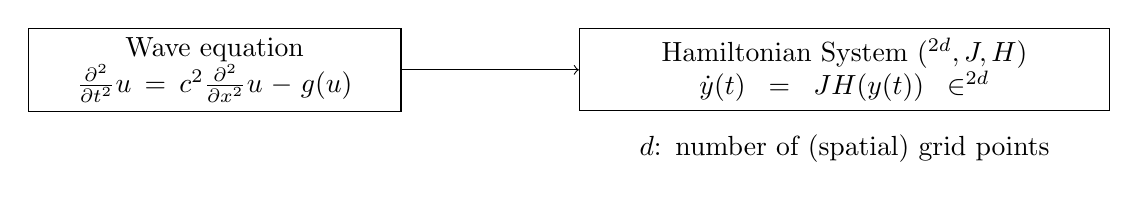
\begin{tikzpicture}
    \node (wave_eq) [draw,text width=4.5cm,align=center] at (0,0)
        {Wave equation\\ 
        $\frac{\partial^2}{\partial t^2} u = 
        c^2 \frac{\partial^2}{\partial x^2} u - g(u)$};

    \node (ham_sys) [draw,text width=6.5cm,align=center] at (8,0)
        {Hamiltonian System $(\R^{2d}, J, H)$\\
        $\dot{y}(t) = J \grad{H}(y(t)) \in \R^{2d}$};

    \node [text width=6.5cm,align=center] at (8,-1)
        {$d$: number of (spatial) grid points};

    \draw [->] (wave_eq) -- (ham_sys);
  \end{tikzpicture}
\end{frame}

\begin{frame}[c]{Linear wave equation}
  $G(u) = g(u) =0$. We use $100$ grid points for the discretization.

  \vspace{0.3cm}
  \begin{itemize}
    \item Training and test data originate from a single trajectory and\\
    are generated with fixed time $t = 0.01$.
    \item Training data corresponds to trajectory for total time $T=0$ to $T=1$.
    \item Test data corresponds to trajectory for total time $T=1$ to $T=10$ (extrapolation).
  \end{itemize}
  
\end{frame}

\begin{frame}[c]
  \begin{figure}
    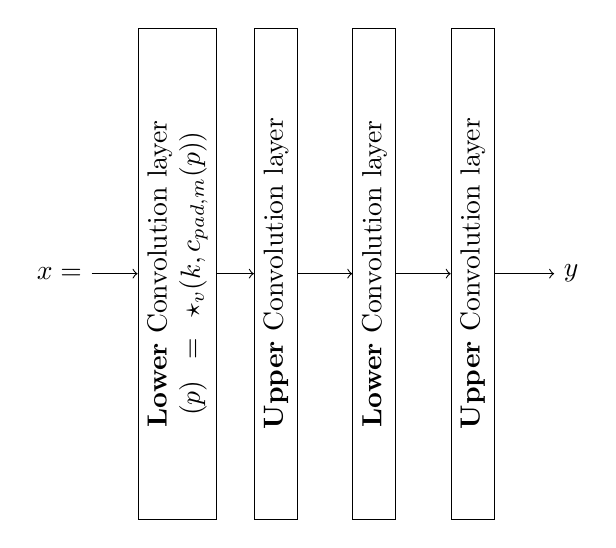
\begin{tikzpicture}
      \node (x) at (0,0) {$x = \qpvec$};

      \node (c1) [draw,text width=6cm,align=center,rotate=90] at (1.5,0) 
        {\textbf{Lower} Convolution layer\\ $\layertf(p) = \star_{\text{v}}(k,c_{\text{pad},m}(p))$};

      \node (c2) [draw,text width=6cm,align=center,rotate=90] at (2.75,0) 
        {\textbf{Upper} Convolution layer};

      \node (c3) [draw,text width=6cm,align=center,rotate=90] at (4,0) 
        {\textbf{Lower} Convolution layer};

      \node (c4) [draw,text width=6cm,align=center,rotate=90] at (5.25,0) 
        {\textbf{Upper} Convolution layer};

      \node (y) at (6.5,0) {$y$};

      \draw[->] (x) -- (c1);
      \draw[->] (c1) -- (c2);
      \draw[->] (c2) -- (c3);
      \draw[->] (c3) -- (c4);
      \draw[->] (c4) -- (y);
    \end{tikzpicture}

    \caption{\bemph{C-SympNet architecture.} 
    All layers with kernel size $3$, constant zero-padding.}
  \end{figure}
\end{frame}

\begin{frame}{Linear wave equation}
  \centering
  \begin{tikzpicture}
    \begin{axis}[
      ymode=log,
      no markers,
      title={Test loss (Linear wave equation)},
      xlabel={Epoch}, xmin=0, xmax=500,
      ylabel={Test loss},
      legend style={nodes={scale=0.75, transform shape}},
      legend cell align=left,
      legend entries={
        CNN,
        C-SympNet (canonical basis),
        C-SympNet (FD basis)
      }
    ]
  
    \addplot[
      color=green
    ] table[x=epoch,y=loss,col sep=comma] {../../data-wave/transport/linear_cnn/sigmoid/test_loss.csv};
  
    \addplot[
      color=blue
    ] table[x=epoch,y=loss,col sep=comma] {../../data-wave/transport/linear_canonical/sigmoid/test_loss.csv};
  
    \addplot[
      color=purple
    ] table[x=epoch,y=loss,col sep=comma] {../../data-wave/transport/linear_fd/sigmoid/test_loss.csv};
      
    \end{axis}
  \end{tikzpicture}
\end{frame}

\begin{frame}{Linear wave equation}
  \centering
  \begin{tikzpicture}
    \begin{axis}[
      title={Displacement $q(t=0,x)$}, ylabel={$q(t=0,x)$},
			legend entries={
				Initial value
      },
      width=0.8*\linewidth, height=\axisdefaultheight,
			xlabel={$x$}, xmin=-0.5, xmax=0.5,
			ymin=-0.3, ymax=0.55, restrict y to domain=-2:2
    ]
      \addplot[
				color=darkgray
			] table[x=x,y=q,col sep=comma] {../../data-wave/transport/exact/q_t0.csv};
    \end{axis}
  \end{tikzpicture}
\end{frame}

\begin{frame}{Linear wave equation}
  \centering
  \begin{tikzpicture}
    \begin{axis}[
      width=0.8*\linewidth, height=\axisdefaultheight,
			xlabel={$x$}, xmin=-0.5, xmax=0.5,
			ymin=-0.3, ymax=0.55, restrict y to domain=-2:2,
      title={Displacement $q(t=3,x)$}, ylabel={$q(t=3,x)$},
			legend style={
				nodes={scale=0.8, transform shape},
				legend cell align=left,
				%legend pos=outer north east
			},
			legend entries={
				CNN,
				C-SympNet (canonical basis),
				C-SympNet (FD basis),
				Ground truth,
			}
    ]
      \addplot[
        color=green
      ] table[x=x,y=q,col sep=comma] {../../data-wave/transport/linear_cnn/sigmoid/q_t3.csv};
    
      \addplot[
        color=blue
      ] table[x=x,y=q,col sep=comma] {../../data-wave/transport/linear_canonical/sigmoid/q_t3.csv};
    
      \addplot[
        color=purple
      ] table[x=x,y=q,col sep=comma] {../../data-wave/transport/linear_fd/sigmoid/q_t3.csv};

      \addplot[
        color=darkgray
      ] table[x=x,y=q,col sep=comma] {../../data-wave/transport/exact/q_t3.csv};
    \end{axis}
  \end{tikzpicture}
\end{frame}

\begin{frame}{Linear wave equation}
  \centering
  \begin{tikzpicture}
    \begin{axis}[
      width=0.8*\linewidth, height=\axisdefaultheight,
			xlabel={$x$}, xmin=-0.5, xmax=0.5,
			ymin=-0.3, ymax=0.55, restrict y to domain=-2:2,
      title={Displacement $q(t=9,x)$}, ylabel={$q(t=9,x)$},
			legend style={
				nodes={scale=0.8, transform shape},
				legend cell align=left,
				%legend pos=outer north east
			},
			legend entries={
				CNN,
				C-SympNet (canonical basis),
				C-SympNet (FD basis),
				Ground truth,
			}
    ]
      \addplot[
        color=green
      ] table[x=x,y=q,col sep=comma] {../../data-wave/transport/linear_cnn/sigmoid/q_t9.csv};
    
      \addplot[
        color=blue
      ] table[x=x,y=q,col sep=comma] {../../data-wave/transport/linear_canonical/sigmoid/q_t9.csv};
    
      \addplot[
        color=purple
      ] table[x=x,y=q,col sep=comma] {../../data-wave/transport/linear_fd/sigmoid/q_t9.csv};

      \addplot[
        color=darkgray
      ] table[x=x,y=q,col sep=comma] {../../data-wave/transport/exact/q_t9.csv};
    \end{axis}
  \end{tikzpicture}
\end{frame}

\begin{frame}[c]{Sine-Gordon}
  Semi-linear wave equation with $G(u) = 1 - \cos(u)$, $g(u) = \sin(u)$ and $c=1$.

  We use $2000$ grid points for the discretization.

  \vspace{0.3cm}
  \begin{itemize}
    \item Training and test data originate from a single trajectory and\\
    are generated with fixed time $t = 0.01$.
    \item Training data corresponds to trajectory for total time $T=0$ to $T=1$.
  \end{itemize}
\end{frame}

\begin{frame}[c]
  \begin{figure}
    \begin{tikzpicture}[node distance=0.3cm]
      \node (c1) [draw,text width=6.5cm,align=center,rotate=90]
        {\textbf{Lower} Convolution layer\\ $T(p) = \star_{\text{v}}(k,\chi_{\text{pad},m}(p))$};

      \node (g1) [draw,text width=6.5cm,align=center,rotate=90,
        right=of c1.south east,anchor=north east,fill=uniSyellow]
        {\textbf{Lower} Convolution Gradient layer};

      \node (c2) [draw,text width=6.5cm,align=center,rotate=90,
        right=of g1.south east,anchor=north east]
        {\textbf{Upper} Convolution layer};

      \node (g2) [draw,text width=6.5cm,align=center,rotate=90,
        right=of c2.south east,anchor=north east,fill=uniSyellow]
        {\textbf{Upper} Convolution Gradient layer};
      
      \node (c3) [draw,text width=6.5cm,align=center,rotate=90,
        right=of g2.south east,anchor=north east]
        {\textbf{Lower} Convolution layer};

      \node (g3) [draw,text width=6.5cm,align=center,rotate=90,
        right=of c3.south east,anchor=north east,fill=uniSyellow]
        {\textbf{Lower} Convolution Gradient layer};

      \node (c4) [draw,text width=6.5cm,align=center,rotate=90,
        right=of g3.south east,anchor=north east]
        {\textbf{Upper} Convolution layer};

      \node (g4) [draw,text width=6.5cm,align=center,rotate=90,
        right=of c4.south east,anchor=north east,fill=uniSyellow]
        {\textbf{Upper} Convolution Gradient layer};

      \node (x) [left=of c1.north] {$x = \qpvec$};
      \node (y) [right=of g4.south] {$y$};

      \draw[->] (x) -- (c1);
      \draw[->] (c1) -- (g1);
      \draw[->] (g1) -- (c2);
      \draw[->] (g2) -- (c3);
      \draw[->] (c3) -- (g3);
      \draw[->] (g3) -- (c4);
      \draw[->] (c4) -- (g4);
      \draw[->] (g4) -- (y);
    \end{tikzpicture}

    \caption{
      \bemph{CG-SympNet architecture.} Convolution layers with kernel size $3$, FD basis
      and symmetric padding. For the Convolution Gradient layers, $\tanh$ is used
      as the activation function.
    }
  \end{figure}
\end{frame}

\begin{frame}{Sine-Gordon}
  \centering
  \begin{tikzpicture}
    \begin{axis}[
      width=0.8*\linewidth, height=\axisdefaultheight,
      no markers,
      xlabel={$x$}, xmin=-25, xmax=25,
			ymin=-1, ymax=10, restrict y to domain=-5:10,
      title={Displacement $q(t=0,x)$}, ylabel={$q(t=0,x)$},
			legend entries={
				Initial value
			}
    ]
      
      \addplot[
          color=darkgray
        ] table[x=x,y=q,col sep=comma] {../../data-wave/sine_gordon/exact/q_t0.csv};
      
    \end{axis}
  \end{tikzpicture}
\end{frame}

\begin{frame}{Sine-Gordon}
  \centering
  \begin{tikzpicture}
    \begin{axis}[
      width=0.8*\linewidth, height=\axisdefaultheight,
      no markers,
      xlabel={$x$}, xmin=-25, xmax=25,
			ymin=-1, ymax=10, restrict y to domain=-5:10,
      title={Displacement $q(t=3,x)$}, ylabel={$q(t=3,x)$},
			legend entries={
				CNN,
				CG-SympNet (tanh),
			  Ground truth,
			}
    ]
      
      \addplot[
        color=green
      ] table[x=x,y=q,col sep=comma] {../../data-wave/sine_gordon/cnn/elu/q_t3.csv};
    
      \addplot[
        color=red
      ] table[x=x,y=q,col sep=comma] {../../data-wave/sine_gordon/gradient/tanh/q_t3.csv};

      \addplot[
        color=darkgray
      ] table[x=x,y=q,col sep=comma] {../../data-wave/sine_gordon/exact/q_t3.csv};
      
    \end{axis}
  \end{tikzpicture}
\end{frame}

\begin{frame}{Sine-Gordon}
  \centering
  \begin{tikzpicture}
    \begin{axis}[
      width=0.8*\linewidth, height=\axisdefaultheight,
      no markers,
      xlabel={$x$}, xmin=-25, xmax=25,
			ymin=-1, ymax=10, restrict y to domain=-5:10,
      title={Displacement $q(t=9,x)$}, ylabel={$q(t=9,x)$},
			legend entries={
				CNN,
				CG-SympNet (tanh),
			  Ground truth,
			}
    ]
      
      \addplot[
        color=green
      ] table[x=x,y=q,col sep=comma] {../../data-wave/sine_gordon/cnn/elu/q_t9.csv};
    
      \addplot[
        color=red
      ] table[x=x,y=q,col sep=comma] {../../data-wave/sine_gordon/gradient/tanh/q_t9.csv};

      \addplot[
        color=darkgray
      ] table[x=x,y=q,col sep=comma] {../../data-wave/sine_gordon/exact/q_t9.csv};
      
    \end{axis}
  \end{tikzpicture}
\end{frame}

\begin{frame}[c]{Summary and Outlook}
  \bemph{Summary:}
  \begin{itemize}
    \item We successfully improved performance of SympNets with batch normalization.
    \item With convolution, we made SympNets applicable for high-dimensional systems
    arising from PDEs.
  \end{itemize}

  \vspace{0.3cm}
  \bemph{Outlook:}
  \begin{itemize}
    \item Convolution in 2D or 3D
    \item Recurrent neural network
  \end{itemize}
\end{frame}